First-order auto-differentiation for a custom module requires the definition of
only two local operations, \emph{forward} and \emph{backward}, whose outputs are
propagated along the computation graph. This modularity facilitates the
extension of gradient backpropagation by new operations, which can then be used
to build networks by composition. To illustrate the principle, we consider a
single module from the net of \Cref{hbp::fig:setting}, depicted in
\Cref{hbp::fig:sketchModule}, in this section\sidenote[][-3\baselineskip]{To
  simplify the presentation, we drop layer indices, choose distinct variable
  names for input and output ($\vx \leftarrow \vz^{(l-1)}$, $\vz \leftarrow
  \vz^{(l)}$, $\vtheta \leftarrow \vtheta^{(l)}$, $f_{\vtheta} \leftarrow
  f^{(l)}_{\vtheta^{(l)}}$) and focus on a single datum.}. The forward pass
$f_{\vtheta}(\vx)$ maps the input $\vx$ to the output $\vz$ by means of the
module parameters $\vtheta$. All quantities are assumed to be vector-shaped
(tensor-valued quantities can be flattened, see
\Cref{def:background::Flattening}). Optimization requires the gradient of the
loss function \wrt the parameters, $\nicefrac{\partial \ell(\vtheta)}{\partial
  \vtheta} = \nabla_{\vtheta}\ell$. We will use the shorthand%
\marginnote{%
  \centering \resizebox{\linewidth}{!}{ \tikzexternalenable \footnotesize
    % A single module with data flow for forward/backward/HBP pass
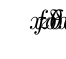
\begin{tikzpicture}
    \node (in)
        [inner sep=0]
        {\tikz \drawMessagesWithArrows{$x$}{$\delta x$}{$\HeCal x$}{\hNodeDistance};};
    \node (module)
         [anchor=south west, inner sep=0]
         at (in.south east)
         {\tikz \drawModuleWithParams{$f$}{16}{$\theta$}{$\delta\theta$}{$\HeCal \theta$};};
    \node (out)
        [inner sep=0, anchor=south west]
        at (module.south east)
         {\tikz \drawMessagesWithArrows{$z$}{$\delta z$}{$\HeCal z$}{\hNodeDistance};};	
\end{tikzpicture} \tikzexternaldisable}
  \vspace{0ex}
  \captionof{figure}{\textbf{Forward pass, gradient backpropagation, and Hessian
      backpropagation for a single module.} Arrows from left to right indicate
    the data flow in the forward pass $\vz = f_{\vtheta}(\vx)$, while the
    opposite orientation indicates the gradient backpropagation by
    \Cref{hbp::equ:gradientBackpropagation}. We suggest to extend this by the
    backpropagation of the Hessian as indicated by
    \Cref{hbp::equ:hessianBackPropagation}.}
  \label{hbp::fig:sketchModule}
}
\begin{align}
  \grad{\cdot}\ell = \frac{\partial \ell(\cdot)}{\partial \vec(\cdot)}\,.
\end{align}
During gradient backpropagation the module receives the loss gradient with
respect to its output, $\grad{\vz}\ell$, from its child. The backward operation
computes gradients \wrt the module parameters and input, $\grad{\vtheta}\ell$
and $\grad{\vx} \ell$ from $\grad{\vz}\ell$. Backpropagation continues by
sending the gradient \wrt the module's input to its parent, which proceeds in
the same way (see \Cref{hbp::fig:setting}). By the chain rule, gradients \wrt an
element $x_{i}$ of the module's input can be computed as $\grad{x_{i}}\ell =
\sum_j (\nicefrac{\partial z_j}{\partial x_i}) \grad{z_{j}}\ell$. The vectorized
version is compactly written in terms of the Jacobian matrix $\jac_{\vx}\vz =
\nicefrac{\partial \vz}{\partial \vx^\top}$
(\Cref{def:background::JacobianVectorVector}), which contains all partial
derivatives of $\vz$ \wrt $\vx$. The arrangement of partial derivatives is
$[\jac_{\vx}\vz ]_{j,i} = \nicefrac{\partial z_j}{\partial x_i}$, such that
\begin{align}
  \grad{\vx} \ell &= \left(\jac_{\vx}\vz\right)^\top \grad{\vz} \ell\,.
             \label{hbp::equ:gradientBackpropagation}
\end{align}
Analogously, the parameter gradients are given by $\grad{\theta_i}\ell = \sum_j
(\nicefrac{\partial z_j}{\partial \theta_i}) \grad{z_j}\ell$, or in vectorized form
$\grad{\vtheta}\ell = \left( \jac_{\vtheta} \vz \right)^\top \grad{\vz}\ell$.
This reflects the symmetry of both $\vx$ and $\vtheta$ acting as input to the
module. Implementing gradient backpropagation thus requires multiplications by
(transposed) Jacobians. We can apply the chain rule a second time to obtain
expressions for second-order partial derivatives of the loss $\ell$
\wrt elements of $\vx$ or $\vtheta$,
\begin{align}
  \label{hbp::equ:chainRuleComponentwise}
  \begin{split}
    \!\frac{\partial^2 \ell}{\partial x_i \partial x_j}
    &=
      \frac{\partial}{\partial x_j}\left( \sum_k \frac{\partial z_k}{\partial x_i}
      \grad{z_k}\ell \right)
    \\
    &= \sum_{k, l} \frac{\partial z_k}{\partial x_i} \frac{\partial^2
      \ell}{\partial z_k \partial z_l} \frac{\partial z_l}{\partial x_j} +\sum_k
      \frac{\partial^2 z_k}{\partial x_i \partial x_j} \grad{z_k}\ell\,,
  \end{split}
\end{align}
by means of $\nicefrac{\partial}{\partial x_j} = \sum_l (\nicefrac{\partial
  z_l}{\partial x_j}) \nicefrac{\partial}{\partial z_l}$ and the product rule.
The first term of \Cref{hbp::equ:chainRuleComponentwise} propagates curvature
information of the output further back, while the second term introduces
second-order effects of the module itself. Using the Hessian matrix
$\gradsquared{\vx}\ell = \nicefrac{\partial^2 \ell}{(\partial \vx^\top \partial
  \vx)}$ of a scalar function \wrt a vector-shaped quantity $\vx$
(\Cref{def:background::Hessian}),
\begin{align}
  \gradsquared{\cdot}\ell(\cdot) = \frac{\partial^2 \ell(\cdot)}{\partial
  \vec(\cdot)^\top \partial \vec(\cdot)}\,,
\end{align}
results in the matrix version of \Cref{hbp::equ:chainRuleComponentwise},
\begin{subequations}
  \label{hbp::equ:hessianBackPropagation}
  \begin{align}
    \gradsquared{\vx}\ell
    &=
      \left( \jac_{\vx} z \right )^\top
      \gradsquared{\vz}\ell
      \ \left( \jac_{\vx} z \right)
      +
      \sum_k \left(\gradsquared{\vx}z_k\right) \grad{z_k}\ell\,.
      \vspace{-\baselineskip}
      \intertext{Note that the second-order effect introduced by the module itself via
      $\gradsquared{\vx}\evz_{k}$ vanishes if all components $[f_\vtheta(\vx)]_{k}$ are
      linear in $\vx$. Because the layer parameters $\vtheta$
      can be regarded as inputs to the layer, they are treated in exactly the same way,
      replacing $\vx$ by
      $\vtheta$ in the above expression,}
      \gradsquared{\vtheta}\ell
    &=
      \left( \jac_{\vtheta} z \right )^\top
      \gradsquared{\vz}\ell
      \ \left( \jac_{\vtheta} z \right)
      +
      \sum_k \left(\gradsquared{\vtheta}z_k\right) \grad{z_k}\ell\,.
  \end{align}
\end{subequations}

\begin{figure*}[t]
  \centering \resizebox{\linewidth}{!} {
    \tikzexternalenable
    \footnotesize
    % Hessian backpropagation scheme for a general feedforward network

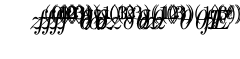
\begin{tikzpicture}
    % first four layers
    \node (in1)
        [inner sep=0]
        {\tikz \drawMessagesWithArrows{$z^{(0)}$}{ }{ }{\hNodeDistance};};
    \node (layer1)
        [anchor=south west, inner sep=0]
        at (in1.south east)
        {\tikz \drawModuleWithParams{$f^{(1)}$}{16}{$\theta^{(1)}$}{$\delta \theta^{(1)}$}{$\HeCal \theta^{(1)}$};};
    \node (out1)
        [inner sep=0, anchor=south west]
        at (layer1.south east)
         {\tikz \drawMessagesWithArrows{$z^{(1)}$}{$\delta  z^{(1)}$}{$\HeCal  z^{(1)}$}{\hNodeDistance};};
    \node (layer2)
        [inner sep=0pt, anchor=south west]
        at (out1.south east)
        {\tikz\drawModuleNoParams{$f^{(2)}$}{5};};
    \node (in2)
        [inner sep=0, anchor=south west]
        at (layer2.south east)
        {\tikz \drawMessagesWithArrows{$z^{(2)}$}{$\delta z^{(2)}$}{$\HeCal  z^{(2)}$}{\hNodeDistance};};
    \node (layer3)
        [anchor=south west, inner sep=0]
        at (in2.south east)
        {\tikz \drawModuleWithParams{$f^{(3)}$}{16}{$\theta^{(3)}$}{$\delta \theta^{(3)}$}{$\HeCal \theta^{(3)}$};};
    \node (out3)
        [inner sep=0, anchor=south west]
        at (layer3.south east)
        {\tikz \drawMessagesWithArrows{$z^{(3)}$}{$\delta  z^{(3)}$}{$\HeCal  z^{(3)}$}{\hNodeDistance};};
    \node (layer4)
        [inner sep=0pt, anchor=south west]
        at (out3.south east)
        {\tikz\drawModuleNoParams{$f^{(4)}$}{5};};	
    \node (dots)
        [xshift=2ex, inner sep=0pt, anchor=west]
         at (layer4.east) {$\dots$};

    % layer after dots
    \node (layer5)
        [xshift=12ex, anchor=south west, inner sep=0]
        at (out3.south east) 
        {\tikz \drawModuleWithParams{$f^{(\ell)}$}{16}{$\theta^{(\ell)}$}{$\delta \theta^{(\ell)}$}{$\HeCal \theta^{(\ell)}$};};
    \node (out4)
        [inner sep=0, anchor=south west]
        at (layer5.south east)
        {\tikz \drawMessagesWithArrows{$z^{(\ell)}$}{$\delta  z^{(\ell)}$}{$\HeCal  z^{(\ell)}$}{\hNodeDistance};};

    % loss layer
    \node (lossLayer) [inner sep=0pt, anchor=south west]
        at (out4.south east)
        {\tikz\drawModuleNoParams{$E$}{5};};
    \node (loss)
        [inner sep=0, anchor=south west]
        at (lossLayer.south east)
        {\tikz \drawMessagesWithArrows{$E$}{ }{ }{\hNodeDistance};};	
\end{tikzpicture}

    \tikzexternaldisable}
  \caption{\textbf{Extension of backpropagation to Hessians.} It yields diagonal blocks of the
    full parameter Hessian. }
  \label{hbp::fig:sketchFCNN}
\end{figure*}

\vspace{-\baselineskip} \Cref{hbp::equ:hessianBackPropagation} is the central
functional expression herein, and will be referred to as the \emph{Hessian
  backpropagation (HBP) equation}. Our suggested extension of gradient
backpropagation is to also send the Hessian $\gradsquared{\vz}\ell$ back through
the graph. To do so, existing modules have to be extended by the HBP equation:
\emph{Given the Hessian $\gradsquared{\vz}\ell$ of the loss \wrt all module
  outputs, an extended module has to extract the Hessians
  $\gradsquared{\vtheta}\ell, \gradsquared{\vx}\ell$ by means of
  \Cref{hbp::equ:hessianBackPropagation}, and forward the Hessian \wrt its input
  $\gradsquared{\vx}\ell$ to the parent module which proceeds likewise.} In this
way, backprop of gradients can be extended to compute curvature information in
modules. This corresponds to BDAs of the Hessian which ignore second-order
derivatives \wrt parameters in different modules. \Cref{hbp::fig:sketchFCNN}
shows the data flow. The computations required in
\Cref{hbp::equ:hessianBackPropagation} depend only on \emph{local quantities}
that are, mostly, already being computed during gradient
backpropagation\sidenote{ By Fa\`a di Bruno's
  formula~\citep{johnson2002FaaDiBruno} higher-order derivatives of function
  compositions are expressed recursively in terms of the composites' lower-order
  derivatives. Recycling these quantities can give significant speedup compared
  to repeatedly applying first-order auto-differentiation, which represents one
  key aspect of our work. }.

Before we proceed, we highlight the following aspects:
\begin{itemize}
\item The BDA of the Hessian need not be PSD. But our scheme can be modified to
  provide PSD curvature matrices by projection onto the positive semi-definite
  cone (see \Cref{hbp::subsec:curvatureMatrices}).

\item Instead of evaluating all matrices during backpropagation, we can define
  matrix-vector products recursively. This yields exact curvature matrix
  multiplications by the block diagonals of the Hessian, the generalized
  Gauss-Newton (\ggn) matrix and the PCH. Multiplications by the first two
  matrices can also be obtained by use of automatic differentiation
  \citep{pearlmutter1994fast,schraudolph2002fast}. We also get access to the PCH
  which, in contrast to the \ggn, considers curvature information introduced by
  the network (see
  \Cref{hbp::subsec:curvatureMatrices}).\sidenote{Implementations of HBP for
    exact matrix-vector products can reuse multiplication by the (transposed)
    Jacobian provided by many ML libraries. The second term
    \Cref{hbp::equ:hessianBackPropagation} needs special treatment though.} For
  standard neural networks, only second derivatives of nonlinear activations
  have to be stored compared to gradient backpropagation.

\item There are approaches \citep{botev2017practical,wei2018bdapch} that
  propagate matrix representations back through the graph to save repeated
  computations in the curvature matrix-vector product. The size of the matrices
  $\gradsquared{\vz^{(l)}}\ell$ passed between layer $l+1$ and $l$ scales
  quadratically in the number of layer $l$'s output features. For convolutional
  layers, the dimension of these quantities exceeds computational budgets. And
  for batched computations, such a matrix has to be backpropagated for every
  datum in the mini-batch. Like previous
  schemes~\citep{botev2017practical,wei2018bdapch}, we introduce additional
  approximations for batch learning in \Cref{hbp::subsec:batchLearning}. A
  connection to existing schemes is drawn in \Cref{hbp::subsec:relation}.
\end{itemize}

HBP is easy to integrate into current ML libraries, so that curvature BDAs
can be provided automatically for novel or existing second-order optimization
methods\sidenote[][-4\baselineskip]{\Eg the matrix-vector products with block-diagonal curvature
  matrices described in this work have been integrated into the \backpack
  library that operates on top of \pytorch and will be presented in
  \Cref{chap:backpack} of this thesis.}. Such methods have repeatedly been
shown to be competitive with first-order
methods~\citep{martens2015optimizing,grosse2016kronecker,botev2017practical,zhang2017blockdiagonal,wei2018bdapch}.

\subsubsection{Relationship to Matrix Differential Calculus}
\label{hbp::sec:MDF}
To some extent, this paper is a re-formulation of earlier results
\citep{martens2015optimizing,botev2017practical,wei2018bdapch} in the framework
of matrix differential calculus \citep{magnus1999MatrixDifferentialCalculus},
leveraged to achieve a new level of modularity. Matrix differential calculus is
a set of notational rules that allow a concise construction of derivatives
without the heavy use of indices. \Cref{hbp::equ:hessianBackPropagation} is a
special case of the matrix chain rule of that framework
(\Cref{def:background::JacobianChainRuleVector,hbp::equ:chainRuleHessians}). A
more detailed discussion of this connection can be found in
\Cref{hbp::sec:matrixDifferentialCalculus} of the Supplements, which also
reviews definitions generalizing the concepts of Jacobian and Hessian in a way
that preserves the chain rule. The elementary building block of our procedure is
a \emph{module} as shown in \Cref{hbp::fig:sketchModule}. Like for gradient
backprop, the operations required for HBP can be tabulated.
\Cref{hbp::table:backpropEquations} provides a selection of common modules. The
derivations, which again leverage the matrix differential calculus framework,
can be found in
\Cref{hbp::sec:examples_fcnn,hbp::sec:examples_loss,hbp::sec:examples_cnn}.

\begin{table*}[t]
  \caption{\textbf{Hessian backpropagation for common modules used in feedforward
    networks.} $\mI$ denotes the identity matrix. We assign matrices to upper-case
    ($\mW, \mX, \dots$) and tensors to upper-case sans serif symbols ($\tW,
    \tX, \dots$).}\label{hbp::table:backpropEquations}
  \centering
  \begin{footnotesize}
    \begin{tabular}{llll}
      \toprule
      \textbf{OPERATION} & \textbf{FORWARD} & \textbf{HBP} (\Cref{hbp::equ:hessianBackPropagation}) & \textbf{DETAILS}
      \\
      \midrule
      % matrix-vector multiplication
      Matrix-vector multiplication & $\vz(\vx, \mW) = \mW\vx$ & $\gradsquared{\vx}\ell = \mW^\top (\gradsquared{\vz}\ell) \mW$\,, & \Cref{hbp::subsec:linearLayerBackwardPass}
      \\
                         & & $\gradsquared{\mW} \ell = \vx \otimes \vx^\top \otimes \gradsquared{\vz}\ell$
      \\[1mm]
      % matrix-matrix multiplication
      Matrix-matrix multiplication & $\mZ(\mX, \mW) = \mW\mX$ & $\gradsquared{\mX} \ell = (\mI \otimes
                                                      \mW)^\top \gradsquared{\mZ} \ell ( \mI \otimes \mW)$\,, & \Cref{hbp::subsec:linearLayerBackwardPass}
      \\[1mm]
                         & & $\gradsquared{\mW} \ell = (\mX^\top \otimes \mI)^\top \gradsquared{\mZ} \ell (\mX^\top \otimes \mI)$
      \\[1mm]
      % addition
      Addition & $\vz(\vx, \vb) = \vx + \vb$ & $\gradsquared{\vx}\ell = \gradsquared{\vb} \ell =\gradsquared{\vz}\ell $ & \Cref{hbp::subsec:linearLayerBackwardPass}
      \\
      % elementwise activation
      Elementwise activation & $\vz(\vx) = \vphi(\vx)$\,,\ \text{s.t.}, & $\gradsquared{\vx}\ell =
                                                     \diag[\vphi'(\vx)]  (\gradsquared{\vz}\ell) \diag[\vphi'(\vx)]$ & \Cref{hbp::subsec:activationBackwardPass}
      \\
                         & $z_i(\vx) = \phi(x_i)$ &  $\phantom{\gradsquared{\vx}\ell =} + \diag[\phi''(\vx) \odot \grad{\vz}\ell]$
      \\
      \midrule
      % residual unit/skip-connection
      Skip-connection & $\vz(\vx, \vtheta) = \vx + \vs(\vx, \vtheta)$ & $\gradsquared{\vx}\ell =
                                                            (\mI + \jac_{\vx}\vs)^\top \gradsquared{\vz}\ell (\mI + \jac_{\vx} \vs)$ & \Cref{hbp::subsec:skipconnectionBackwardPass}
      \\
                         &     & $\phantom{\gradsquared{\vx}\ell =} + \sum_k (\gradsquared{\vx} s_k) \grad{z_k}\ell$\,,
      \\
                         & & $\gradsquared{\vtheta}\ell = (\jac_{\vtheta} \vs)^\top \gradsquared{\vz}\ell (\jac_{\vtheta} \vs)$
      \\
                         & & $\phantom{\gradsquared{\vtheta}\ell } + \sum_k (\gradsquared{\vtheta} s_k) \grad{z_k}\ell$
      \\
      \midrule
      % reshape/view operation
      Reshape/view & $\tZ(\tX)=
                     \mathrm{reshape}(\tX)$ & $\gradsquared{\tZ}\ell = \gradsquared{\tX}\ell$ & \Cref{hbp::subsec:HBPReshape}
      \\
      % extraction operator
      Index select/map $\pi$ & $\vz(\vx) = \mPi \vx\, ,$ $\emPi_{j,\pi(j)} =
                               1\,, $ & $\gradsquared{\vx}\ell = \mPi^\top(\gradsquared{\vz}\ell)\mPi$ %(same as
                               % matrix-vector mul.\ with $W$)
                                                                                                    & \Cref{hbp::subsec:HBPIndexSelect}
      \\
      % convolution
      Convolution & $\tZ(\tX, \tW) = \tX
                    \star \tW$\,, & $\gradsquared{\llbracket \tX \rrbracket}\ell =
                                           (\mI \otimes \mW)^{\top} \gradsquared{\mZ} \ell (\mI \otimes \mW)$
                                                                                                    & \Cref{hbp::subsec:convolutions}
      \\
                         & $\mZ(\mW, \llbracket\tX\rrbracket) = \mW
                           \llbracket \tX \rrbracket$\,, & $\gradsquared{\mW} \ell = (\llbracket
                                                                  \tX \rrbracket^\top \otimes \mI)^\top \gradsquared{\mZ} \ell (\llbracket
                                                                  \tX \rrbracket^\top \otimes \mI)$
      \\
      \midrule
      % square loss
      Square loss & $\ell(\vf, \vy) = \nicefrac{1}{C}(\vy-\vf)^\top (\vy - \vf)$ & $\gradsquared{\vf}\ell = \nicefrac{2}{C} \mI$ & \Cref{hbp::subsec:mselossBackwardPass}
      \\
      % cross-entropy loss
      Softmax cross-entropy & $\ell(\vf, y) = - \onehot(y)^\top \log\left[
                              \vp(\vf)\right]$ & $\gradsquared{\vf}\ell = \diag [\vp(\vf)]- \vp(\vf)
                                             \vp(\vf)^\top$ & \Cref{hbp::subsec:crossentropylossBackwardPass}
      \\
      \bottomrule
    \end{tabular}
  \end{footnotesize}
\end{table*}

%%% Local Variables:
%%% mode: latex
%%% TeX-master: "../thesis"
%%% End:
